% ==============================================================================================================
\section{Confronto tra ansatze per il calcolo dell’energia}\label{sez:contronti-UCC}

In questa sezione vengono confrontate le prestazioni di vari ansatz per il calcolo dell’energia dello stato fondamentale della molecola di LiH a diversi valori della distanza internucleare. Gli ansatz analizzati comprendono diverse varianti di $q$-UCC, tra cui $q$-UCCS, $q$-UCCD, $q$-UCCSD, e $q$-pUCCD, oltre a EfficientSU(2), di tipo \inglese{hardware-efficient}. L’obiettivo è valutare le differenze di prestazioni in termini sia di accuratezza energetica sia di complessità circuitale. I calcoli sono stati eseguiti su simulatori ideali, quindi senza rumore hardware, ma possono comunque offrire un’indicazione del potenziale di ciascun metodo per applicazioni pratiche.

Coerentemente con quanto esposto nelle Sezioni~\ref{sez:quantum-coupled-cluster} e \ref{sez:hardware-efficient}, ci si attende di osservare prestazioni migliori in quegli ansatz che considerano un maggior numero di configurazioni: $q$-UCCSD e $q$-UCCD.  Tuttavia, se da un lato è chiaro che $q$-UCCSD raggiunga il risultato più accurato, lo stesso non si può dire per le soluzioni intermedie: sarà rilevante osservare fino a che punto possano competere in precisione le alternative meno costose, come $q$-pUCCD e EfficientSU(2). Ques'ultimo, in particolare, dovrebbe risultare l’ansatz meno costoso - fra quelli analizzati~- in termini di operazioni richieste. Per quanto riguarda $q$-UCCS, ci si aspetta una \inglese{performance} più debole, dal momento che le eccitazioni singole includono un basso numero di configurazioni.

La Figura~\ref{fig:LiH-confronti} riporta il confronto tra i valori energetici calcolati per ciascun ansatz. Per contestualizzare il miglioramento ottenuto grazie alla considerazione della correlazione elettronica (sez. \ref{sez:post-HF}), viene inclusa anche l’energia ottenuta con il metodo di Hartree-Fock (sez. \ref{subsec:Hartree-Fock}). Al di sotto, la Tabella~\ref{tab:energie-e-circuiti} riporta i valori dell’energia per ciascun ansatz alle distanze di legame ($E_0$) e a lungo raggio ($E_\infty$), oltre che la massima deviazione riscontrata dal valore FCI, $\Delta E_{\text{max}}$, fornendo una visione d'insieme sulle differenze tra gli approcci sia in termini di accuratezza che di complessità del circuito.

\begin{figure}[H]
    \centering
    \hspace{-0.9cm}
    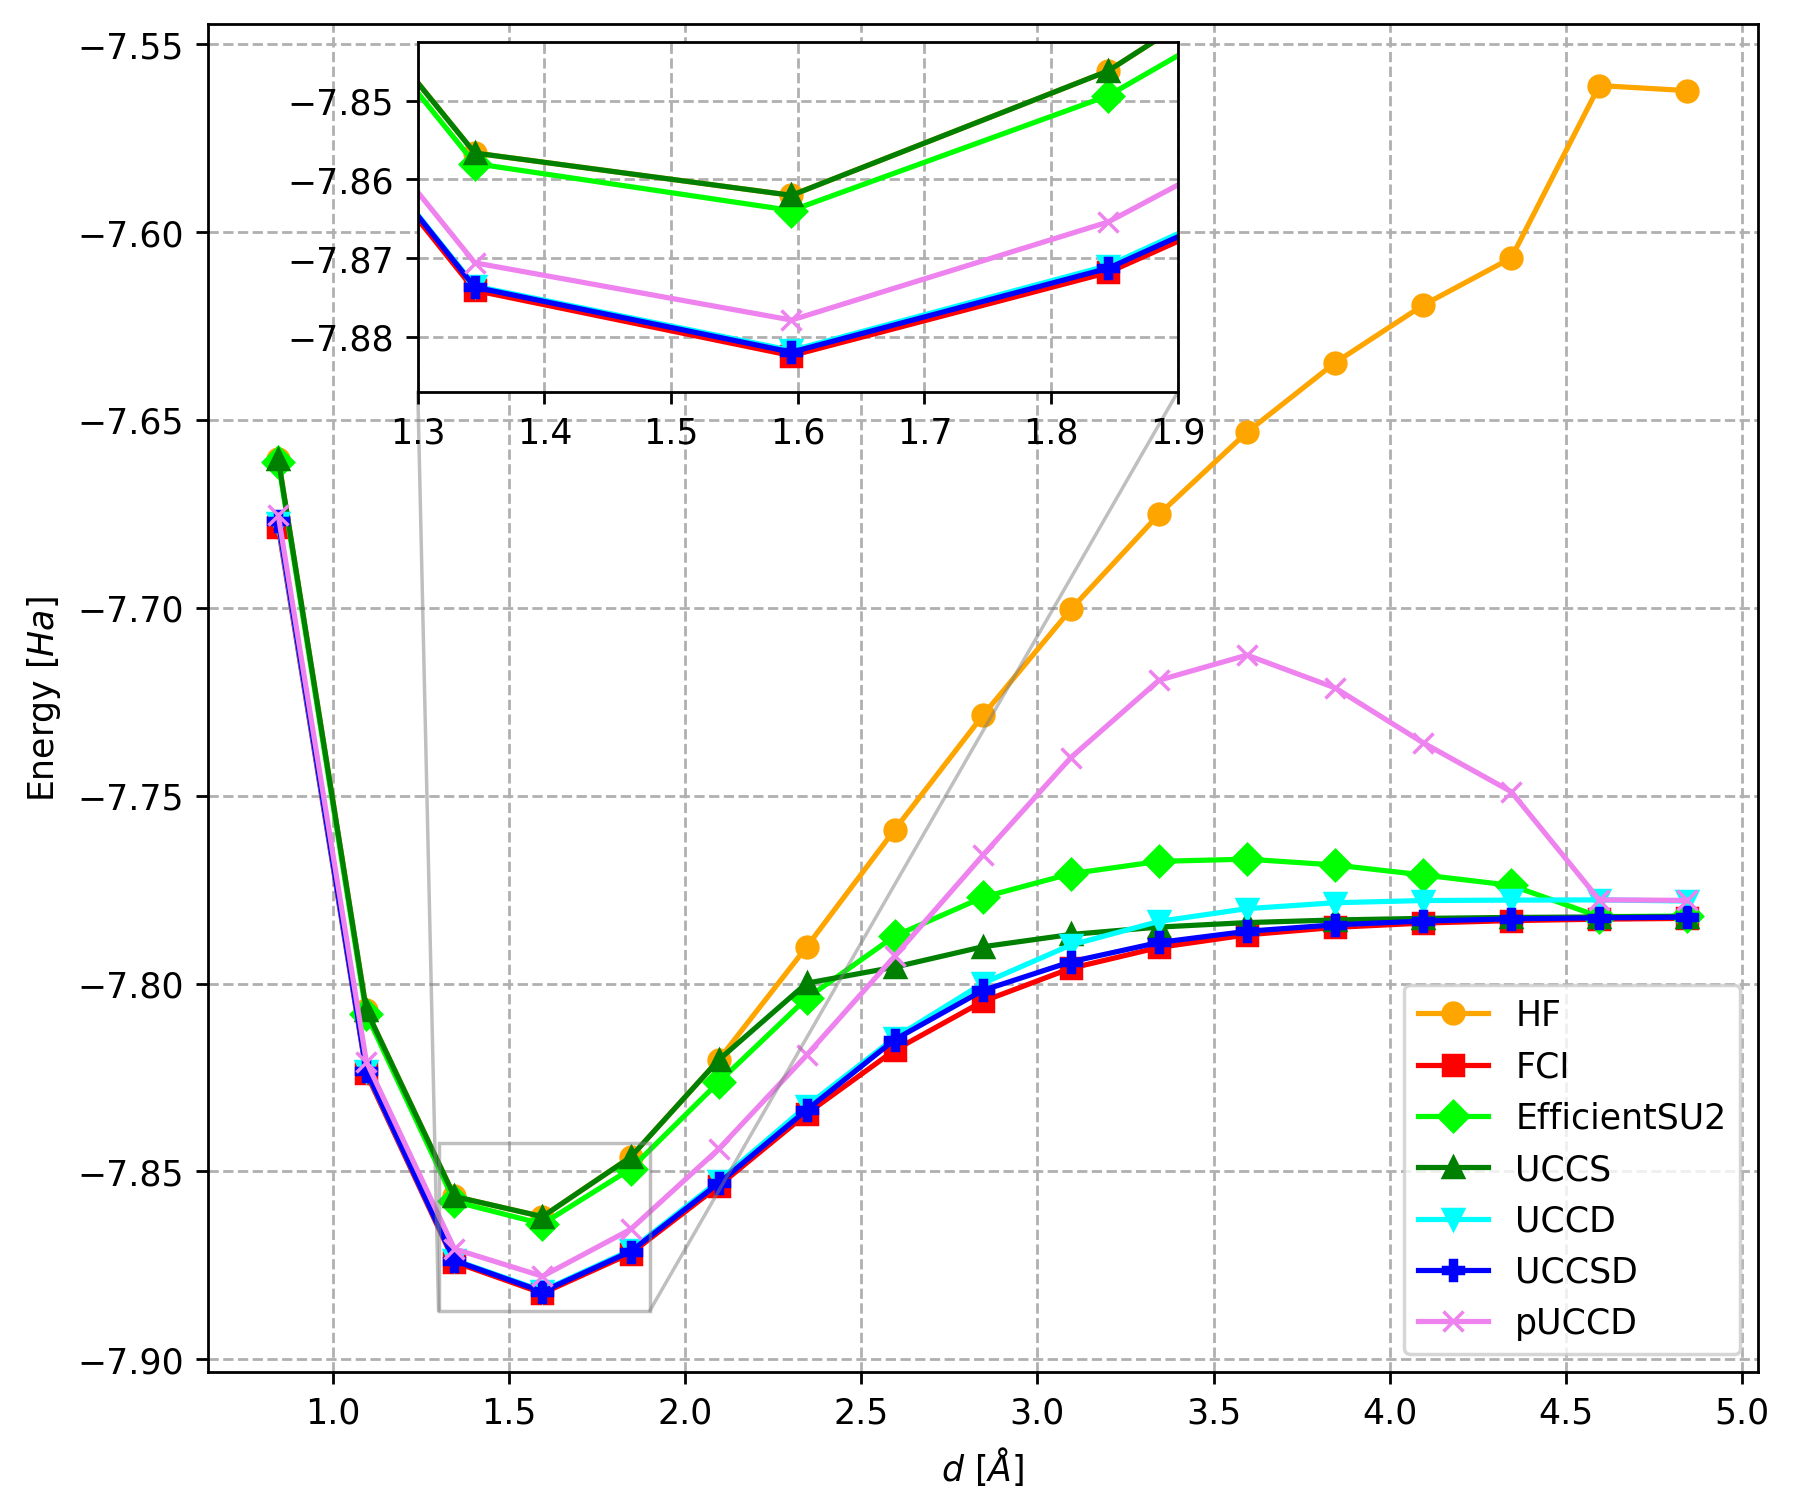
\includegraphics[width=.6\linewidth]{Immagini/Capitolo_3/LiH_ground.png}
    \caption{LiH: confronto tra ansatze.}
    \label{fig:LiH-confronti}
\end{figure}

% Please add the following required packages to your document preamble:
% \usepackage[table,xcdraw]{xcolor}
% Beamer presentation requires \usepackage{colortbl} instead of \usepackage[table,xcdraw]{xcolor}
% Please add the following required packages to your document preamble:
% \usepackage[table,xcdraw]{xcolor}
% Beamer presentation requires \usepackage{colortbl} instead of \usepackage[table,xcdraw]{xcolor}
\begin{table}[H]
    \centering
    \begin{tabular}{|c|c|c|c|c|c|c|}
    \hline
    \textbf{Metodo}                                                 & \textbf{Depth} & \textbf{CNOT} & \textbf{Parametri} & \textbf{$E_0$} & \textbf{$E_\infty$} & \textbf{$\Delta E_{\text{max}}$} \\ \hline
    \textbf{\color[HTML]{CB0000} FCI}          & /              & /             & /                  & -7.8824             & -7.7827                  & /                                     \\ \hline
    \textbf{\color[HTML]{32CB00} EfficientSU2} & 21             & 40            & 80                 & -7.8640             & -7.7820                  & 0.03                                  \\ \hline
    \textbf{\color[HTML]{036400} $q$-UCCS}     & 71             & 80            & 8                  & -7.8620             & -7.7820                  & 0.04                                  \\ \hline
    \textbf{\color[HTML]{34CDF9} $q$-UCCD}     & 2032           & 1536          & 16                 & -7.8817             & -7.7780                  & 0.007                                 \\ \hline
    \textbf{\color[HTML]{3531FF} $q$-UCCSD}    & 2098           & 1616          & 24                 & -7.8820             & -7.7823                  & 0.003                                 \\ \hline
    \textbf{\color[HTML]{D952D8} $q$-pUCCD}    & 511            & 384           & 4                  & -7.8779             & -7.7779                  & 0.07                                  \\ \hline     
\end{tabular}
\caption{Energie calcolate in hartree (Ha) e dimensioni dei circuiti.}
\label{tab:energie-e-circuiti}
\end{table}

Prima di tutto, si può notare che le previsioni HF si discostano molto dal valore di FCI, specialmente a grandi distanze. È quindi evidente che, per quanto semplice, l'approssimazione di Hartree-Fock non restituisce valori sufficientemente accurati.
Gli ansatze $q$-UCCSD, praticamente sovrapposto a FCI, e $q$-UCCD si confermano i metodi \inglese{} più precisi, con il primo che mostra una distanza massima in energia dal valore di riferimento di soli 0.003 hartree, e il secondo che si mantiene nello stesso ordine di grandezza con 0.007 Ha. La deviazione di $q$-UCCS invece è paragonabile a quella di EfficientSU(2), entrambe quasi dieci volte maggiori dei circuiti precedenti. Tuttavia, è interessante notare che, sempre in termini di deviazione massima, l'ansatz \inglese{hardware-efficient} risulta generalmente più accurato di $q$-pUCCD, con quest'ultimo che mostra grandi differenze nella descrizione della dissociazione, arrivando a circa 0.07 Ha al di sopra del valore di riferimento.  
Quindi, in linea con le attese, gli ansatze $q$-UCC più strutturati tendono a fornire valori di energia più accurati, a fronte di circuiti più profondi. Sempre in Tabella~\ref{tab:energie-e-circuiti} sono riportate la profondità e il numero di porte CNOT per ciascun circuito; ad esempio, $q$-UCCSD ha una \inglese{depth} di 2098, con 1616 porte CNOT, risultando il più complesso tra quelli considerati; $q$-UCCD è simile, essendo fondamentalmente lo stesso circuito privato dei 71 \inglese{layers} di $q$-UCCS. $q$-pUCCD, avendo un numero significativamente inferiore di configurazioni incluse, scende a 511, un quarto rispetto ai precedenti. D’altra parte, EfficientSU(2) mostra una profondità di appena 21 e nonostante ciò, per lo meno a grandi distanze, non mostra discrepanze energetiche sensibilmente più ampie.

La Figura~\ref{fig:energie-profondità-colorbar} illustra il confronto tra le energie stimate e la profondità dei circuiti per ciascuna forma variazionale, sempre alle due distanze di $E_0$ (fig.~\ref{fig:energie-profondità-colorbar}a) e $E_\infty$ (fig.~\ref{fig:energie-profondità-colorbar}b). Ogni punto rappresenta un ansatz, con il colore che varia in funzione della profondità del circuito, nonché la complessità di implementazione.

Alla distanza di equilibrio si osserva che i metodi $q$-UCCSD e $q$-UCCD si avvicinano maggiormente al valore di riferimento FCI, ma presentano una profondità di circuito significativamente più elevata. All'infinito la situazione arriva quasi all'inversione, con i più semplici EfficientSU(2) e $q$-UCCS che scendono al di sotto di $q$-UCCD. 

\begin{center}
    \begin{figure}[H]%
        \subfloat[\centering Alla distanza di legame]{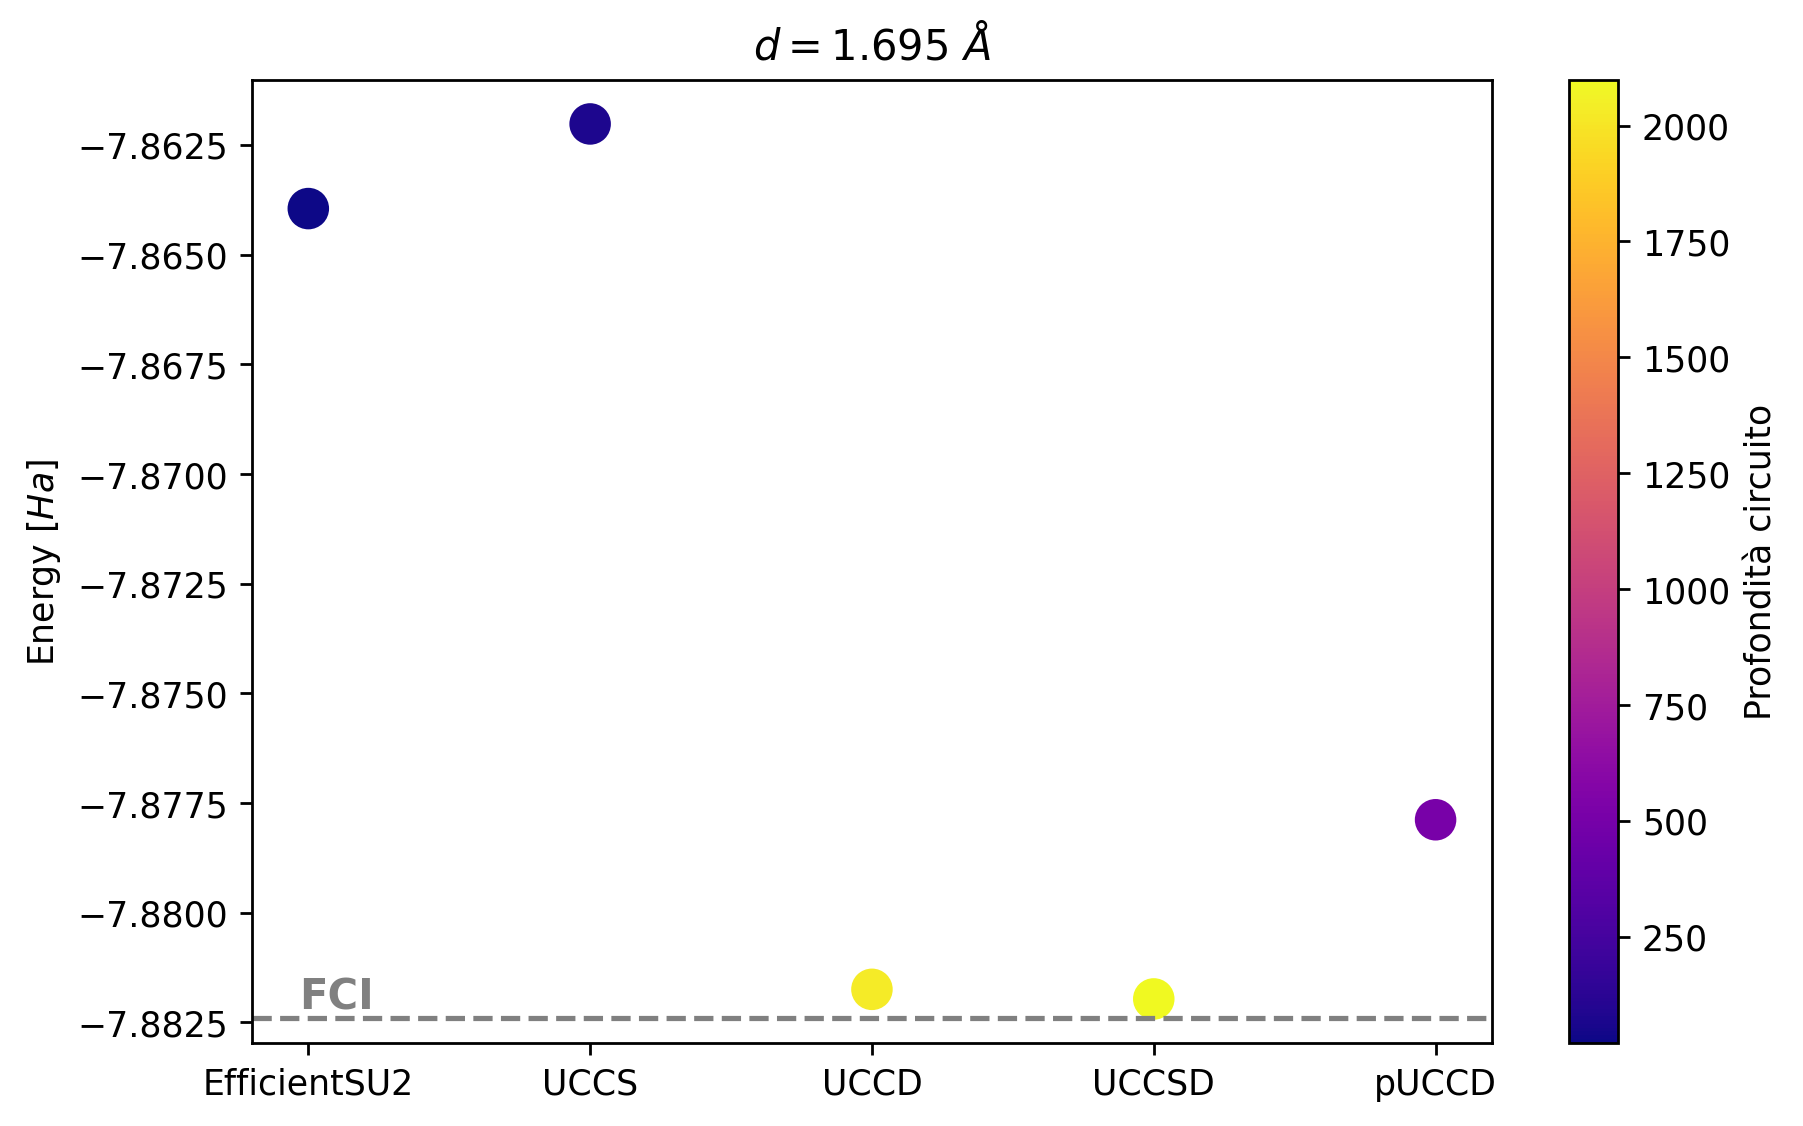
\includegraphics[width=.5\linewidth]{Immagini/Capitolo_3/ground.png}}%
        \hfill
        \subfloat[\centering A grande distanza]{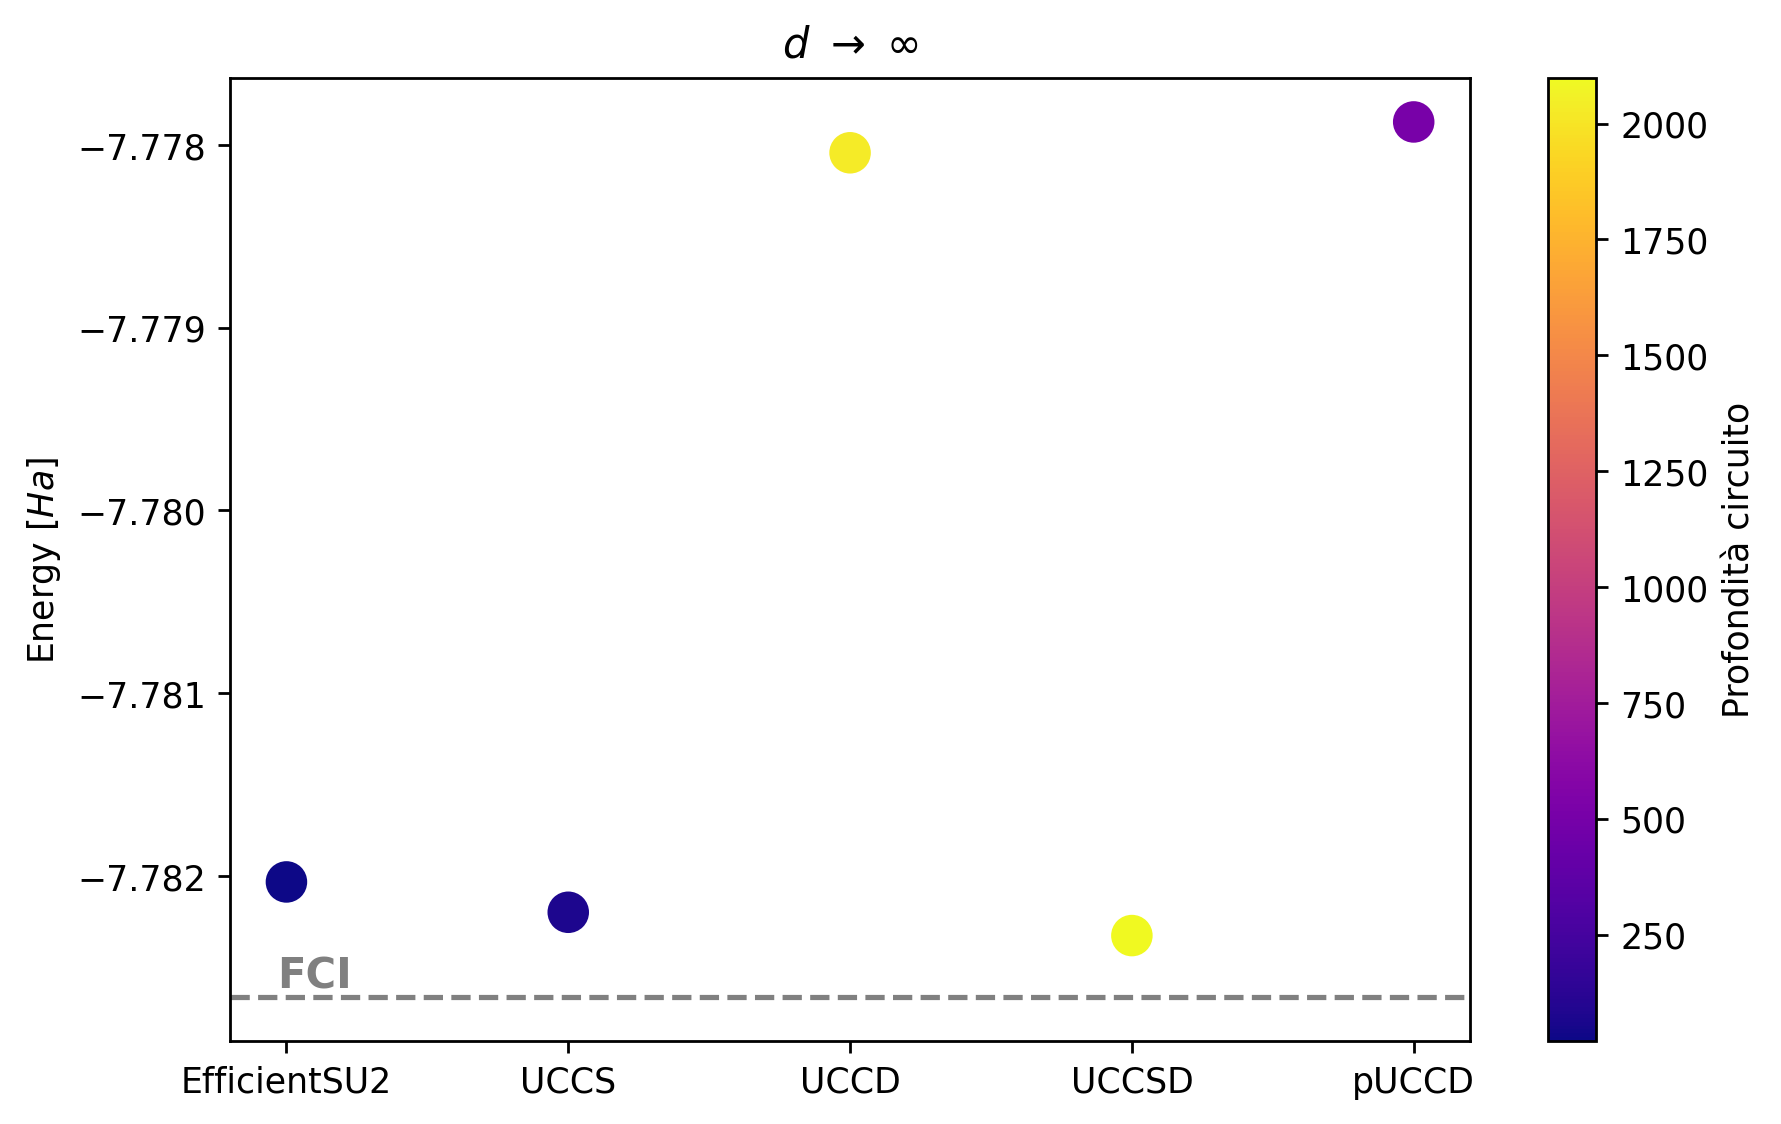
\includegraphics[width=.5\linewidth]{Immagini/Capitolo_3/dissociazione.png}}%
        \caption{LiH: confronto energie e profondità dei circuiti.}%
        \label{fig:energie-profondità-colorbar}%
    \end{figure}
\end{center}

I comportamenti osservati riscontrati possono essere spiegati considerando i tipi di correlazioni elettroniche che ciascuna forma variazionale riesce a rappresentare. Alla distanza di equilibrio, dove gli atomi sono vicini e legati, sono richiesti metodi in grado di descrivere con precisione le complesse interazioni elettroniche che caratterizzano il legame chimico. Qui gli ansatze che includono eccitazioni doppie, come $q$-UCCD e $q$-UCCSD, catturano meglio le influenze reciproche e pertanto forniscono stime di energia più accurate.
In fase di dissociazione, invece, gli elettroni diventano progressivamente più indipendenti. La correlazione elettronica è meno intensa e un metodo semplice come $q$-UCCS può descrivere in modo adeguato la situazione, anche se include solo eccitazioni singole. Questo perché, all’infinito, la mancanza di interazione tra gli elettroni fa sì che la descrizione dell’energia totale non richieda una struttura complessa.
$q$-UCCSD, che comprende eccitazioni singole e doppie, è in grado di bilanciare le esigenze di complessità del legame e la semplicità della dissociazione, combinando i vantaggi degli altri due.

Infine, $q$-pUCCD mostra contemporaneamente una sovrastima nel valore dell'energia all'equilibrio e, poiché anch'esso trascura le eccitazioni del primo ordine, anche nel valore di $E_\infty$. Tuttavia, esiste una tecnica capace di portare un miglioramento significativo alle stime prodotte da $q$-pUCCD, soprattutto per quanto riguarda la descrizione della dissociazione: l'\textbf{ottimizzazione orbitale}, introdotta nella Sezione~\ref{subsec:pUCCD}, che mitiga in parte l'iniziale esclusione delle \inglese{singles}.

% --------------------------------------------------------------------------------------------------------------
\subsection{Analisi del processo di ottimizzazione}

Per ogni ansatz, il processo di ottimizzazione dell’energia a una distanza fissa di $d=1.595$ \AA~è stato valutato analizzando:
\begin{itemize}
    \item la varianza dei valori campionati durante l’ottimizzazione;
    \item la massima distanza tra il valore di convergenza e i valori provati.
\end{itemize}

La Figura~\ref{fig:LiH-UCC-ottimizzazione} illustra l’andamento dell’ottimizzazione per ciascun ansatz, mentre i valori numerici sono riportati nella Tabella \ref{tab:ottimizzazione}:

\begin{figure}[H]
    \centering
    \hspace{-0.9cm}
    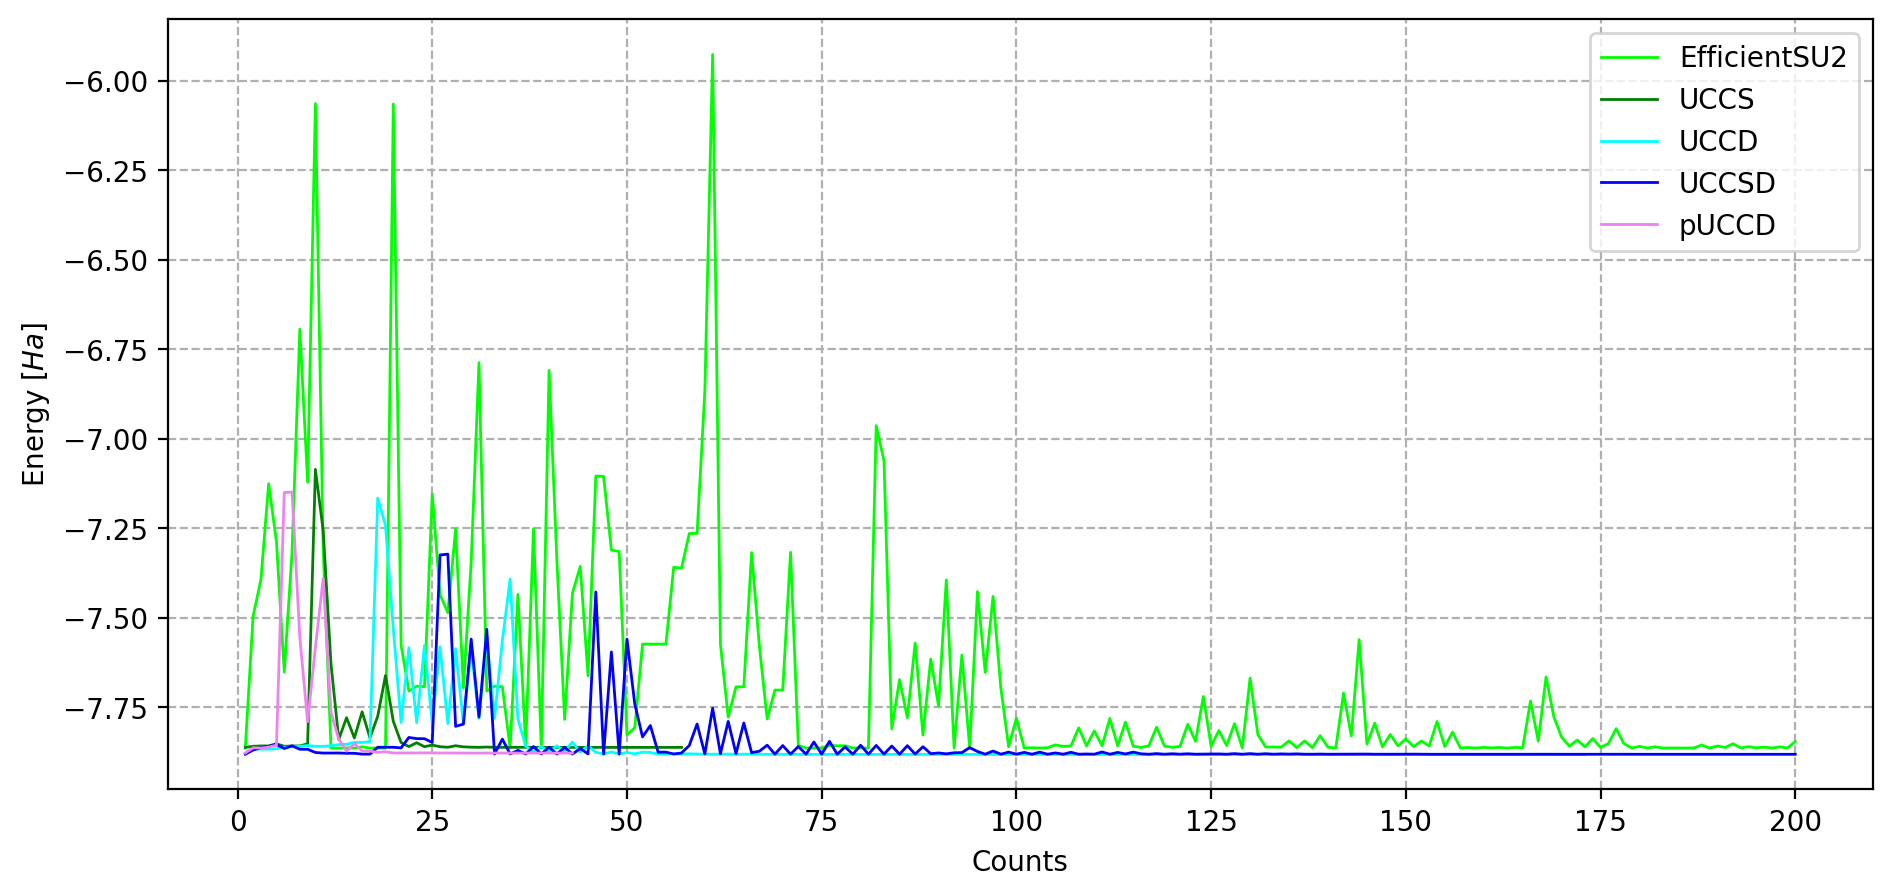
\includegraphics[width=.8\linewidth]{Immagini/Capitolo_3/ottimizzazione.png}
    \caption{LiH: processo di ottimizzazione a $d=1.595$ \AA.}
    \label{fig:LiH-UCC-ottimizzazione}
\end{figure}


\begin{table}[H]
    \centering
    \begin{tabular}{|c|c|c|}
    \hline
    \textbf{Ansatz}                              & \textbf{Varianza (Ha$^2$)} & \textbf{Massima $\Delta E$ (Ha)} \\ \hline
    {\color[HTML]{32CB00} \textbf{EfficientSU2}} & 0.1       & 1.9        \\ \hline
    {\color[HTML]{036400} \textbf{UCCS}}         & 0.02      & 0.8        \\ \hline
    {\color[HTML]{34CDF9} \textbf{UCCD}}         & 0.01      & 0.7        \\ \hline
    {\color[HTML]{3531FF} \textbf{UCCSD}}        & 0.006     & 0.6        \\ \hline
    {\color[HTML]{D952D8} \textbf{pUCCD}}        & 0.03      & 0.7        \\ \hline
\end{tabular}
\caption{Varianza e massima distanza nel processo di ottimizzazione.}
\label{tab:ottimizzazione}
\end{table}


L'ansatz \inglese{hardware-efficient} mostra una varianza significativamente più alta (0.1~Ha$^2$) rispetto alle varianti $q$-UCC, suggerendo che esso vada ad esplorare un’area più ampia dello spazio dei parametri durante l’ottimizzazione. Data la sua natura \inglese{problem agnostic}, ciò potrebbe significare che nella ricerca vengono incluse anche delle regioni non interessanti in senso fisico, portando a una minore stabilità. D'altra parte, negli ansatze $q$-UCC la varianza è decisamente più bassa: da tre volte minore per $q$-pUCCD ($0.03$~Ha) fino a quasi venti volte più piccola per $q$-UCCSD ($0.006$~Ha). Ciò potrebbe indicare un’esplorazione più localizzata intorno al minimo energetico, con un maggiore focus sulle regioni fisicamente significative. Tuttavia, questa focalizzazione non garantisce necessariamente una maggiore stabilità: anche in simulazioni ideali è stato necessario ripetere più volte il processo di ottimizzazione per ottenere risultati consistenti, segnalando un'alta sensibilità ai parametri iniziali e rappresentando una sfida per applicazioni su dispositivi rumorosi.

Lo stesso comportamento si osserva nella distanza massima tra valore di convergenza e valori provati. In questo caso, EfficientSU(2) presenta una distanza massima molto alta, di circa $2$~Ha. Questo è coerente con una maggiore ampiezza nell’esplorazione dello spazio dei parametri, che potrebbe risultare vantaggiosa per evitare minimi locali, ma può aumentare la possibilità di risultati devianti. Al contrario, $q$-UCCSD presenta la distanza minore (0.6 Ha), indicativa di una ricerca più mirata e di una maggiore costanza nella convergenza verso il minimo globale. Tuttavia, proprio questa localizzazione dei minimi può rendere più probabile che l’ottimizzazione si arresti prematuramente, prima di raggiungere il vero minimo assoluto, specialmente in presenza di rumore. Lo stesso discorso si applica anche alle altre varianti \inglese{Coupled Cluster}, che mostrano diverge massime sempre nell'ordine dei decimi di hartree: $0.7$~Ha per $q$-UCCD e $q$-pUCCD, $0.8$~Ha per $q$-UCCS.

In generale, gli ansatze con una varianza più bassa e una distanza massima minore tendono a raggiungere il minimo più rapidamente, mentre EfficientSU(2) potrebbe richiedere più iterazioni a causa della maggiore ampiezza esplorativa. Anche se il numero di iterazioni e il tempo di ottimizzazione dipendono dalla potenza di calcolo disponibile, questo rimane un dato interessante per valutare l’efficienza degli ansatze in contesti pratici.

